\documentclass[UTF8]{ctexart}
\usepackage[a4paper,margin=2.5cm]{geometry}
\usepackage{amsmath}
\usepackage{amssymb}
\usepackage{booktabs}
\usepackage{graphicx}
\usepackage{natbib}
\usepackage{caption}
\setcounter{secnumdepth}{0}

\title{面向风险敏感型任务无关外骨骼辅助的可靠性感知生物关节力矩估计}
\author{匿名投稿}
\date{}

\begin{document}
\maketitle

\begin{abstract}
任务无关外骨骼控制器将可穿戴传感器的历史序列直接映射为生物关节力矩，因此即使模型在标称条件下的预测误差较低，传感器故障仍可能传播至辅助指令。本文将在参与者、任务和传感器故障均发生偏移时的部署可靠性，建模为一个基于验证集标定的风险—效用决策问题：故障证据应当改变控制指令，同时避免不必要地抑制有效辅助。

我们提出一种因果多信号监控器，将概率关节力矩估计、学习得到的预测一致性信号以及针对特定故障机制的完整性检查相结合，并进一步将经过标定的时间步级风险映射为连续力矩门控。信号归一化、检测器选择和门控调节均仅使用验证数据。参与者互斥的评测涵盖分布内任务、留出任务、已报告的训练期故障，以及模型训练和检测器选择均未使用的三种故障生成器。在三个随机种子上，对于未见故障生成器，冻结后的检测器在分布内任务和留出任务上分别达到 $0.842$ 和 $0.778$ 的宏平均 AUROC。相对于采用相同数据划分的确定性 TCN，可靠性训练使干净试验的 RMSE 在分布内任务和留出任务上分别增加 $0.011$ Nm/kg 和 $0.021$ Nm/kg。在验证数据上选定的保守工作点处，门控使已报告故障场景中受到反向力矩作用的有效时间步比例平均降低约 $0.7$ 个百分点，同时在干净试验中保留未门控估计器 $96.1\%$ 的同向力矩。在 15 折留一参与者实验中，逐参与者的降低量为 $0.44$ 个百分点（$95\%$ bootstrap 置信区间 $[0.23, 0.67]$），且对每位参与者都为正。结果表明，部署可靠性应通过故障判别能力、控制后果和标称效用保留程度进行联合评估。
\end{abstract}

\section{引言}

动力下肢外骨骼能够降低运动消耗，并帮助步态受损人群，但控制器需要在使用者切换活动时判断应当提供何种辅助 \citep{young2017state,kim2019exosuit,awad2017soft,siviy2023opportunities}。基于模式的控制器从固定任务集合中作出这一判断 \citep{camargo2021classification,kang2022classification}，因此难以扩展到动作过渡和非结构化运动。任务无关控制则从可穿戴传感器估计髋、膝生物关节力矩，并以这一连续生理状态辅助周期性、瞬态和非结构化动作 \citep{molinaro2022hip,molinaro2024unifies,molinaro2024task}。公开生物力学数据与领域适应进一步减少了设备专用数据的采集需求 \citep{scherpereel2023dataset,scherpereel2025domain}。其他研究根据人体响应对力矩曲线进行个性化，或在仿真中学习通用辅助策略 \citep{zhang2017humanloop,slade2022personalizing,luo2024simulation}。

更广的任务覆盖范围并不意味着每次部署预测都可靠。冻结的数据流、漂移、突发丢包或模态不同步都可能破坏原本熟悉的试验。预测力矩会进入力矩生成流程，因此这些错误可能削弱有效辅助，甚至使其方向反转。干净数据上的 RMSE 无法揭示这类孤立事件，预测不确定性也未必能够检测局部仍然合理的保持值或缓慢传感器漂移 \citep{ovadia2019trust}。此外，检测到异常并不能直接说明执行器应如何响应。本文关注的问题是：任务无关力矩估计器能否检测多种传感器故障，并在不过度抑制有效辅助的情况下作出响应？

我们使用在合成故障上训练的因果多头 TCN 回答这一问题。网络预测关节力矩、数据相关不确定性、故障概率、干净输入重建和短期传感器值。独立监控器将这些输出与因果完整性检查结合，在不接触测试数据的情况下选择输入，并将时刻级风险映射为连续力矩门控。实验采用参与者互斥的数据划分，将任务偏移与未见故障生成器分开，并同时报告故障检测、反向力矩和保留辅助。

\section{相关工作}

\paragraph{任务无关外骨骼控制。}
传统控制器先推断离散运动模式或步态相位，再应用任务专用力矩策略 \citep{camargo2021classification,kang2022classification}，难以扩展到瞬态和非结构化动作。基于力矩的控制则把生物关节力矩的即时估计作为连续控制状态：先用于变速辅助与跨条件、与受试者无关的髋力矩预测 \citep{shepherd2022deep,molinaro2022hip}，随后成为多种行走条件下的统一控制表示 \citep{molinaro2024unifies}，最终在不显式分类任务的情况下实现髋膝协调辅助 \citep{molinaro2024task}。本文沿用其传感配置、预测目标和控制变换。这些工作评估的是标称条件下的估计准确率；其传感器消融衡量移除某一模态的影响，但不估计传感器健康状态、不标定部署风险，也不在检测到故障时改变辅助。

\paragraph{数据效率与领域偏移。}
力矩标签依赖动作捕捉与测力台，且与设备绑定，因此 \citet{scherpereel2025domain} 用 CycleGAN 把开源生物力学数据转换到目标传感器域，减少所需的目标域标签。人在环与便携式调节实现的个性化 \citep{zhang2017humanloop,slade2022personalizing} 以及仿真训练策略 \citep{luo2024simulation} 同样作用于部署之前。这些方法改变估计器或辅助曲线的获取方式；本文处理的是部署之后在目标设备上遇到的观测损坏。监控器可以套在领域适应后的估计器外部，但本文不重新实现其转换模型。

\paragraph{不确定性、异常与选择性预测。}
异方差回归把输入相关的观测噪声与预测均值分开 \citep{kendall2017uncertainties}，MC dropout 和深度集成近似认知不确定性 \citep{gal2016dropout,lakshminarayanan2017ensembles}，但两者在分布偏移下都可能失准 \citep{ovadia2019trust}。不确定性感知的踝关节辅助按 OOD 估计开关辅助，针对的是动作新颖性而非结构化传感器故障 \citep{tourk2025uncertainty}。对多变量时间序列，重建误差和变量间关系变化能提供预测方差遗漏的证据 \citep{song2023memto,dai2024sarad}，这正是引入机理专用通道的动机。选择性预测允许模型在预期误差高时拒绝输出，并以风险—覆盖率曲线评估 \citep{geifman2019selectivenet}；辅助控制器无法在不规定执行器行为的前提下拒绝输出，因此本文把标定风险转换为连续增益，并在面向控制的约束下选择该映射。

\section{问题定义}

令 $\mathbf{x}_{1:T}\in\mathbb{R}^{C\times T}$ 表示因果输入窗口，其中包含足部、小腿和大腿 IMU、鞋垫以及髋膝编码器的单侧测量。目标 $\mathbf{y}_{t}\in\mathbb{R}^{2}$ 为按体重归一化的髋膝生物关节力矩。部署时，未知损坏 $f\in\mathcal{F}$ 可能改变观测并产生 $\widetilde{\mathbf{x}}_{1:T}$。我们希望得到预测器 $\widehat{\mathbf{y}}_t$ 和可靠性门控 $g_t\in[0,1]$，使指令力矩
\begin{equation}
    \boldsymbol{\tau}^{\mathrm{cmd}}_t
    = g_t\,\mathcal{C}(\widehat{\mathbf{y}}_{1:t})
\end{equation}
在干净输入下保留有效辅助，并在任务偏移或传感器故障下抑制有害指令。$\mathcal{C}$ 表示基线中的力矩缩放、延迟、滤波和饱和流程。

评估需要同时覆盖力矩保真度、故障区分能力以及安全性与有效性之间的平衡，任何单一指标都不足以完整描述性能。

\section{方法}

图~\ref{fig:overview-zh} 概括本文方法的三个部分：可穿戴输入流及其可能出现的故障、带有可靠性预测头和完整性检查的共享因果估计器，以及由验证数据标定的风险到连续力矩门控的映射。

\begin{figure*}[t]
\centering
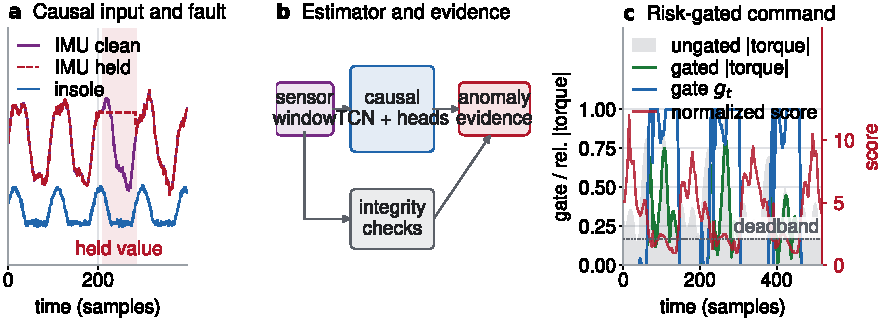
\includegraphics[width=\textwidth]{figures/fig_method_overview.pdf}
\caption{方法概览。（a）可穿戴传感器提供因果输入流，其中可能出现局部仍然合理的故障；波形为示意，阴影区间为保持值故障。（b）共享因果 TCN 同时预测髋膝力矩和互补的学习可靠性证据，完整性检查针对特定故障机理；标定、检测器选择和门控调节只使用验证数据。（c）种子 7 模型在注入 \texttt{encoder\_dropout} 的同分布测试窗口上的真实逐时刻导出：融合风险超过死区时门控衰减基线力矩指令，风险回落后门控立即恢复为 1。}
\label{fig:overview-zh}
\end{figure*}

\subsection{可靠性感知因果 TCN}

使用训练参与者的逐通道均值 $\mathbf{c}$ 与标准差 $\mathbf{v}\in\mathbb{R}^{C}$ 对每个观测进行归一化：
\begin{equation}
    \mathbf{z}_t=(\mathbf{x}_t-\mathbf{c})\oslash
    \max(\mathbf{v},10^{-6}),
\end{equation}
其中 $\oslash$ 表示逐元素除法。按照 \citet{molinaro2024task} 和 \citet{bai2018tcn}，共享编码器包含 $L=5$ 个残差块。每个残差块包含两个因果卷积，卷积核大小为 $k=5$，膨胀率为 $2^{\ell-1}$，并使用权重归一化、ReLU 和空间 dropout。感受野为
\begin{equation}
    H=1+2(k-1)\sum_{\ell=1}^{L}2^{\ell-1}=249
\end{equation}
个采样点，因此训练和评估时排除每个窗口前 $H-1$ 个输出。

五个 $1\!\times\!1$ 预测头分别输出力矩均值 $\boldsymbol{\mu}_t$、对数方差 $\mathbf{s}_t$、二元故障 logit $a_t$、干净输入重建 $\widehat{\mathbf{z}}_t$ 和 $h$ 步预测 $\overline{\mathbf{z}}_{t+h\mid t}$。我们将 $\mathbf{s}_t$ 截断到 $[-8,5]$，并定义对角预测分布
\begin{equation}
    p(\mathbf{y}_t\mid\widetilde{\mathbf{x}}_{1:t})
    = \mathcal{N}\!\left(\boldsymbol{\mu}_t,
      \operatorname{diag}(\exp\mathbf{s}_t)\right).
\end{equation}

\subsection{故障增强多任务学习}

每个训练窗口从干净数据或六种故障中采样，包括鞋垫缺失、编码器丢失、IMU 偏置、丢包、IMU 卡死和传感器延迟。算子 $\widetilde{\mathbf{x}}=\mathcal{A}_f(\mathbf{x};\boldsymbol{\xi})$ 将缺失模态置零，施加按方差缩放的偏置斜坡，在丢包后保持前值，或对不同模态施加不同延迟以形成异步。

每种生成器的强度和作用模态均固定：鞋垫组和编码器组直接置零；小腿 IMU 施加 $0.25$ 倍通道标准差的偏置斜坡，大腿 IMU 施加 $0.35$ 的轴向尺度误差；丢包对所有组以概率 $0.15$ 独立保持前值；IMU 卡死冻结足部 IMU；传感器延迟对所有组平移 $10$ 个采样点（$50$~ms），并按足、小腿、大腿、鞋垫、编码器分别乘以 $1.0$、$1.6$、$0.6$、$2.0$、$1.2$，使各模态相互异步而非整体滞后。每种故障占满整个窗口，因此下文的故障标签 $b_f$ 在窗口内恒定。三种留出生成器沿用相同强度但机理不同：突发丢包在速率 $p$ 下丢弃长度 $\max(2,\operatorname{round}(2+24p))$ 的连续段，部分丢包对每个通道独立抽掩码，抖动延迟每个窗口在标称值的 $[0.5,1.5]$ 倍内重抽。

令 $m_{jt}$ 表示力矩标签是否有效，并令 $b_f=\mathbb{I}[f\neq\mathrm{clean}]$。带掩码的异方差损失为
\begin{equation}
\begin{aligned}
\mathcal{L}_{\mathrm{mom}}
&=\frac{1}{2\sum_{j,t}m_{jt}}\sum_{j,t}m_{jt}\,\ell_{jt},\\
\ell_{jt}&=s_{jt}+(y_{jt}-\mu_{jt})^2\exp(-s_{jt}).
\end{aligned}
\end{equation}
力矩头接收 $\widetilde{\mathbf{x}}$，但仍以干净的 $\mathbf{y}$ 为目标，使模型能够在故障后仍保留足够信息时维持估计。故障头使用时刻级二元交叉熵：
\begin{equation}
\begin{aligned}
\mathcal{L}_{\mathrm{fault}}=-\frac{1}{|\Omega|}\sum_{t\in\Omega}
\big[&b_f\log\sigma(a_t)\\
&+(1-b_f)\log(1-\sigma(a_t))\big],
\end{aligned}
\end{equation}
其中 $\Omega$ 包含至少一个关节标签有效的时刻。

辅助头恢复未损坏的归一化序列，而不是复现损坏输入：
\begin{align}
\mathcal{L}_{\mathrm{rec}} & = \operatorname{MSE}_{\Omega}
\left(\widehat{\mathbf{z}}_t(\widetilde{\mathbf{x}}),\mathbf{z}_t(\mathbf{x})\right),\\
\mathcal{L}_{\mathrm{pred}} & = \operatorname{MSE}_{\Omega}
\left(\overline{\mathbf{z}}_{t+h\mid t}(\widetilde{\mathbf{x}}_{1:t}),\mathbf{z}_{t+h}(\mathbf{x})\right).
\end{align}
完整目标函数为
\begin{equation}
    \mathcal{L}=\mathcal{L}_{\mathrm{mom}}+
    \lambda_f\mathcal{L}_{\mathrm{fault}}+
    \lambda_r\mathcal{L}_{\mathrm{rec}}+
    \lambda_p\mathcal{L}_{\mathrm{pred}},
\end{equation}
其中 $(\lambda_f,\lambda_r,\lambda_p)=(0.2,0.1,0.1)$。重建损失更新共享编码器，而预测分支在 $\mathbf{h}_t$ 处停止梯度，使该分支仅作为时间探针。

\subsection{互补完整性信号}

不同故障影响不同的信号属性，因此监控器考虑八个候选信号。学习得到的信号包括故障概率 $q_t^{\mathrm{fault}}=\sigma(a_t)$、平均偶然不确定性尺度 $q_t^{\mathrm{ale}}=\frac{1}{2}\sum_j\exp(s_{jt}/2)$、重建与预测残差，以及可选的认知不确定性尺度。对于模态组 $G$，残差分数为
\begin{align}
q_t^{\mathrm{rec}} &= \max_G\frac{1}{|G|}\sum_{c\in G}
(\widehat z_{ct}-\widetilde z_{ct})^2,\\
q_{t+h}^{\mathrm{pred}} &= \max_G\frac{1}{|G|}\sum_{c\in G}
(\overline z_{c,t+h\mid t}-\widetilde z_{c,t+h})^2.
\end{align}
时刻 $t$ 作出的预测只能在目标于 $t+h$ 到达后评分。等价地，时刻 $u$ 的风险比较 $\overline{\mathbf{z}}_{u\mid u-h}$ 与 $\widetilde{\mathbf{z}}_u$。前 $h$ 个采样点的该通道被置零，从而保持指令时刻的因果性。认知不确定性尺度是随机 dropout 前向传播或集成成员之间力矩均值标准差的关节平均。

三个因果统计量覆盖学习头可能遗漏的故障特征。停滞性是近似不变通道比例的滑动值。一致性是一减去对应 IMU 轴差分信号之间滚动相关系数绝对值的均值。漂移取各模态通道斜率平均值中的最大值。一致性和漂移仅作为离线诊断通道，不进入指令时刻门控。

\subsection{验证集标定的故障检测}

对验证窗口 $i$，在有效时刻 $\Omega_i$ 上对每个通道取平均，得到 $Q_{ik}=|\Omega_i|^{-1}\sum_{t\in\Omega_i}q_{it}^{k}$。检测器参考值由干净验证窗口定义：
\begin{equation}
    \rho_k^{\mathrm{det}}=\operatorname{Quantile}_{0.9}
    \left(\{Q_{ik}:i\in\mathcal{V}_{\mathrm{clean}}\}\right).
\end{equation}
对信号子集 $S$，融合分数为
\begin{equation}
    R_i^{\mathrm{det}}(S) = \max_{k\in S}
    Q_{ik}/\max(\rho_k^{\mathrm{det}},10^{-6}).
\end{equation}
我们只使用验证故障枚举至多包含三个通道的子集。给定验证故障 AUROC $A_f(S)$，选择准则为
\begin{equation}
    J_{\mathrm{det}}(S)=\operatorname{mean}_f A_f(S)
    +0.25\min_f A_f(S)-0.002(|S|-1).
\end{equation}
第二项奖励最难故障上的性能，最后一项偏向较小的子集。在测试前固定 $S$ 和 $\rho_k^{\mathrm{det}}$。突发丢包、独立部分通道缺失和随机延迟抖动均不参与训练或检测器选择。

\subsection{有效性感知辅助门控}

故障检测 AUROC 与控制风险具有不同作用。指令时刻风险使用当前配置可用的因果时刻级通道 $\mathcal{K}_{\mathrm{gate}}=\{\mathrm{fault},\mathrm{ale},\mathrm{rec},\mathrm{pred},\mathrm{epi},\mathrm{stale}\}$：
\begin{equation}
    r_t=\max_{k\in\mathcal{K}_{\mathrm{gate}}}
    q_t^k/\max(\rho_k^{\mathrm{gate}},10^{-6}).
\end{equation}
我们共享检测器尺度 $\rho_k^{\mathrm{gate}}:=\rho_k^{\mathrm{det}}$，以保持窗口级与时刻级分数可比较；该值并非时刻分数的分位数。干净的留出任务验证试验和指定验证故障用于标定死区 $d$ 与软化参数 $\gamma$。

风险被转换为连续增益：
\begin{equation}
g_t = \operatorname{clip}_{[0,1]}\!\left(
1-\frac{r_t-(1+d)}{\gamma}\right),
\end{equation}
其中 $d$ 定义死区，$\gamma$ 控制衰减的平滑程度。当 $r_t\leq1+d$ 时，$g_t=1$；超过该区域后，$g_t$ 线性下降。

从 $d_0=0.1$ 出发，我们设置
\begin{equation}
    d=\min\!\left(d_{\max},\max\left[d_0,
    \operatorname{Quantile}_{0.9}(r^{\mathrm{val\text{-}OOD}})-1\right]\right),
\end{equation}
其中 $d_{\max}=2$，计算使用验证参与者的干净留出任务试验。随后搜索 $\gamma\in\{0.25,0.5,1,2,4,8\}$。可行参数需保留至少 $95\%$ 的干净同向力矩，满足干净条件下的反向力矩容差，并且不增加验证故障下的反向力矩。以 $\kappa_{\mathrm{clean}}$ 记门控前后的干净保留比，并在验证故障上取平均，$\bar\delta$ 记相对反向力矩降幅 $\min(1,\max(0,1-w^{\mathrm{gated}}/w^{\mathrm{ungated}}))$、$\bar\kappa$ 记故障保留比，则可行参数按
\begin{equation}
    J_{\mathrm{gate}} = \kappa_{\mathrm{clean}} + 2\bar\delta + 0.25\,\bar\kappa
\end{equation}
排序：安全项占主导，但不能靠直接关断门控换取；不可行参数被剔除。

基线控制变换 $\mathcal{C}$ 分别以 $0.20$ 和 $0.15$ 缩放髋膝估计力矩，施加设定的关节延迟和 6-Hz 低通滤波，并将力矩截断到 $0.45$ Nm/kg。门控指令为 $\boldsymbol{\tau}^{\mathrm{cmd}}_t=g_t\mathcal{C}(\boldsymbol{\mu}_{1:t})$。该策略衰减来自不可靠估计的指令，但不能替代独立的执行器饱和与硬件安全限制。

\section{实验协议}

\subsection{数据、划分与比较方法}

我们使用任务无关控制器所公开的外骨骼传感器和生物关节力矩数据 \citep{molinaro2024task,scherpereel2023dataset}，统一重采样到 $200$~Hz，因此一个采样点为 $5$~ms，预测步长 $h=1$ 即一个控制周期。输入包含 25 个单侧通道，分为五个模态组 $G$：足、小腿、大腿 IMU（各 6 通道，三轴陀螺加三轴加速度）、鞋垫（3）、髋膝编码器（4）；输入消融中的动作通道构成第六组。目标为以 Nm/kg 表示的右侧髋膝力矩。15 名参与者中 11 名用于训练、2 名验证、2 名测试，跳跃、切向运动、举重和弓步保留为任务 OOD；预处理、标定、检测器选择和门控调节均不使用测试参与者。留一参与者分析轮换全部 15 名参与者，共 15 折，每折以前一名参与者作验证。主要基线是在相同划分上训练的确定性、无增强 TCN。公开的 Nature 检查点使用不同划分，因此只作为背景参照。消融按顺序加入故障增强、概率回归、重建和预测，并额外分析 dropout、集成、动作输入、故障强度和留一参与者测试。

\subsection{指标与实现}

我们报告 RMSE、MAE、$R^2$、高斯 NLL、不确定性与误差相关性、区间覆盖率与校准误差，以及单通道和融合故障 AUROC。

控制回放指标以理想指令 $\boldsymbol{\tau}^{\star}=\mathcal{C}(\mathbf{y})$ 为基准，即把\textbf{真实}力矩送入同一变换 $\mathcal{C}$。当标签有效且 $|\tau^{\star}_n|>0.02$ Nm/kg 时，该关节—时刻对 $n$ 记为\textbf{活跃}；活跃集 $\mathcal{A}$ 只由真实力矩决定，因此门控前后完全相同，不会被衰减缩小。记 $u_n=\tau^{\mathrm{cmd}}_n$，反向力矩比例 $w$ 与保留同向力矩 $\kappa$ 为
\begin{align}
w &= \tfrac{1}{|\mathcal{A}|}\textstyle\sum_{n\in\mathcal{A}}
     \mathbb{I}[u_n\tau^{\star}_n<0],\\
\kappa &= \frac{\sum_{n\in\mathcal{A}}\max(0,\,u_n\operatorname{sgn}\tau^{\star}_n)}
       {\sum_{n\in\mathcal{A}}|\tau^{\star}_n|}，
\end{align}
另外报告反向步上 $|u_n|$ 的峰值与指令加加速度的平均绝对值。由于 $u_n=g_t\mathcal{C}(\boldsymbol{\mu})_n$ 且 $g_t\geq0$，缩放不改变符号：$w$ 的任何下降都只来自 $g_t$ 恰好取 0 的时刻，而 $\kappa$ 就是为此付出的代价。所以两者必须同时报告，且都无法靠单纯压低门控改善。

一阶执行器代理还估计净力矩 RMS 和功相关指标；这些指标只用于离线相对比较，不代表实测代谢收益。模型包含五个 80 通道 TCN 块，卷积核大小为 5，dropout 为 0.15，窗口长度为 768，步幅为 384，并屏蔽前 248 个输出。使用 Adam 训练 20 个 epoch，学习率为 $10^{-3}$，随机种子为 7、13 和 23，报告均值、标准差和配对种子差异。三个种子只刻画训练随机性，因此主安全结论的区间估计改由 15 折留一参与者实验给出，对逐参与者的反向力矩降低量报告基于折的百分位 bootstrap $95\%$ 置信区间（$10{,}000$ 次重采样，固定随机种子）。我们不报告逐场景显著性检验：十个场景乘两个划分再乘若干指标，未校正的检验族无法解释，三个种子上的多重比较校正又几乎没有检验力，因此逐场景数值只作描述性报告，确认性结论只依赖那一个预先指定的被试间置信区间。

\section{结果}

除非另有说明，表中结果均为随机种子 7、13 和 23 的均值与标准差，所有检测器和门控选择均固定于验证数据。

\subsection{力矩准确率与校准}

表~\ref{tab:accuracy-zh} 比较了未损坏试验上的本文模型与划分匹配的确定性 TCN。在 ID 任务上，可靠性训练使 RMSE 从 $0.1616\pm0.0008$ 变为 $0.1726\pm0.0017$ Nm/kg，配对差值为 $+0.0110\pm0.0024$。对应的 OOD 数值为 $0.2319\pm0.0050$ 和 $0.2531\pm0.0023$ Nm/kg，配对差值为 $+0.0213\pm0.0045$。概率模型在 ID 和 OOD 任务上的覆盖率 ECE 分别为 $0.033\pm0.017$ 和 $0.028\pm0.010$。因此，可靠性感知模型以部分干净准确率为代价提高故障可靠性，而不是同时改善两个指标。公开的 Nature 检查点只作为背景参照，因为其参与者和任务划分与本文不匹配。

\begin{table}[t]
\centering
\small
\begin{tabular}{lcccc}
\toprule
方法 & RMSE & R2 & NLL & ECE\\
\midrule
\multicolumn{5}{l}{ID 任务}\\
确定性 TCN & $0.162\pm0.001$ & $0.798\pm0.002$ & -- & --\\
本文方法 & $0.173\pm0.002$ & $0.770\pm0.005$ & $-1.453\pm0.034$ & $0.033\pm0.017$\\
\addlinespace[2pt]
\multicolumn{5}{l}{留出任务（OOD）}\\
确定性 TCN & $0.232\pm0.005$ & $0.751\pm0.011$ & -- & --\\
本文方法 & $0.253\pm0.002$ & $0.704\pm0.005$ & $-1.063\pm0.022$ & $0.028\pm0.010$\\
\bottomrule
\end{tabular}
\caption{未见参与者上的干净力矩估计与校准，数值为三个随机种子的均值 $\pm$ 标准差。RMSE 单位为 Nm/kg。RMSE、NLL 和 ECE 越低越好，R2 越高越好。确定性 TCN 不定义 NLL 和 ECE。}
\label{tab:accuracy-zh}
\end{table}

\subsection{任务偏移下的故障检测}

图~\ref{fig:detection-zh} 与表~\ref{tab:detection-zh} 给出冻结融合检测器及其候选通道在代表性故障上的 AUROC。对于报告的六个训练期故障，融合检测器在 ID 和留出任务上的宏平均 AUROC 分别为 $0.849\pm0.005$ 和 $0.773\pm0.002$。对于未见的突发丢包、部分通道缺失和延迟抖动生成器，对应宏平均 AUROC 为 $0.842\pm0.010$ 和 $0.778\pm0.004$。一致性是最强单一信号，在部分通道缺失和 IMU 停滞两种故障上于 ID 和 OOD 均达到 $1.000$ AUROC；IMU 偏置则是最困难的融合故障，AUROC 分别为 $0.502$ 和 $0.504$。逐故障报告能够避免聚合 AUROC 掩盖系统性检测失败。

\begin{figure}[t]
\centering
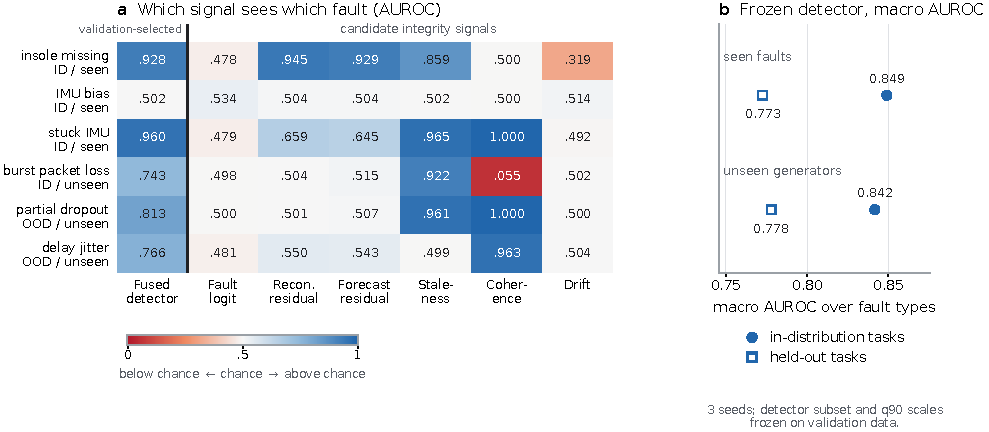
\includegraphics[width=\linewidth]{figures/fig_detection_taxonomy.pdf}
\caption{各故障机理在互补信号上的可检测性。（a）每个候选信号与冻结融合检测器的干净—故障 AUROC；融合列单独置于左侧，其信号子集和尺度仅由验证数据确定。单元格颜色以随机水平为中心发散，蓝色高于随机，红色低于随机，中性中点为 $0.500$。行标注给出故障名称及其生成器是否参与训练。（b）冻结检测器在故障类型上的宏平均 AUROC，圆形为分布内任务，方形为留出任务（三个随机种子均值）。}
\label{fig:detection-zh}
\end{figure}

\begin{table*}[t]
\centering
\scriptsize
\setlength{\tabcolsep}{2.5pt}
\begin{tabular}{llccccccc}
\toprule
划分 & 故障 & 融合 & Logit & 重建 & 预测 & 停滞 & 一致性 & 漂移\\
\midrule
ID & 鞋垫缺失 & $0.928\pm0.013$ & $0.478\pm0.055$ & $0.945\pm0.014$ & $0.929\pm0.013$ & $0.859\pm0.001$ & $0.500\pm0.000$ & $0.318\pm0.002$\\
ID & IMU 偏置 & $0.502\pm0.001$ & $0.534\pm0.003$ & $0.504\pm0.003$ & $0.504\pm0.002$ & $0.502\pm0.000$ & $0.500\pm0.000$ & $0.514\pm0.000$\\
ID & IMU 停滞 & $0.960\pm0.000$ & $0.479\pm0.009$ & $0.659\pm0.009$ & $0.645\pm0.006$ & $0.965\pm0.000$ & $1.000\pm0.000$ & $0.492\pm0.000$\\
ID & 突发丢包（未见） & $0.743\pm0.020$ & $0.498\pm0.001$ & $0.504\pm0.000$ & $0.515\pm0.002$ & $0.922\pm0.002$ & $0.055\pm0.004$ & $0.502\pm0.001$\\
OOD & 部分通道缺失（未见） & $0.813\pm0.003$ & $0.500\pm0.000$ & $0.501\pm0.001$ & $0.507\pm0.001$ & $0.961\pm0.001$ & $1.000\pm0.000$ & $0.500\pm0.000$\\
OOD & 延迟抖动（未见） & $0.766\pm0.010$ & $0.481\pm0.000$ & $0.550\pm0.002$ & $0.543\pm0.002$ & $0.499\pm0.001$ & $0.963\pm0.010$ & $0.504\pm0.002$\\
\bottomrule
\end{tabular}
\caption{代表性的干净与故障 AUROC。“未见”表示相应生成器未参与模型训练和检测器选择，其他故障行因篇幅省略。}
\label{tab:detection-zh}
\end{table*}

\subsection{安全性与有效性的平衡}

图~\ref{fig:safety-zh} 与表~\ref{tab:safety-zh} 比较应用冻结门控前后的本文估计器；$w$ 的变化是有效时刻占比之差，因此 $-0.0074$ 即 $-0.74$ 个百分点。

\begin{figure}[t]
\centering
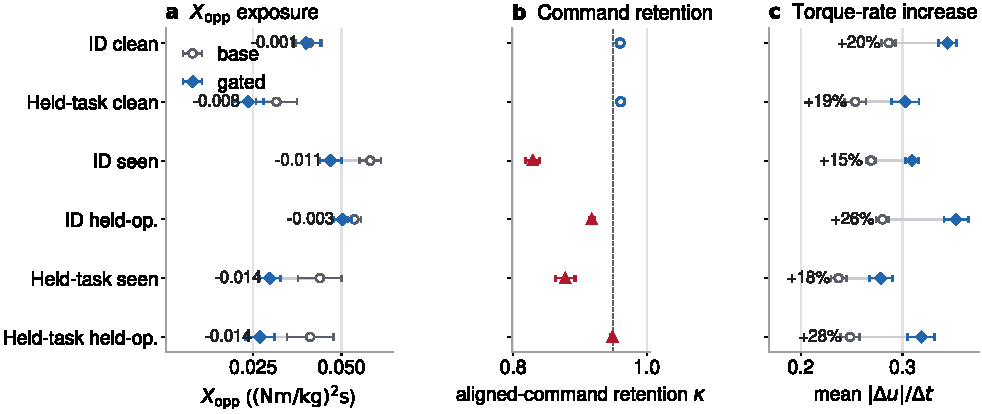
\includegraphics[width=\linewidth]{figures/fig_safety_utility.pdf}
\caption{冻结门控的控制后果。（a）配对标记比较各场景门控前后的反向力矩比例，直接标注给出以百分点表示的配对差值。（b）安全—效用平面将反向力矩降幅与保留同向力矩对应，空心圆为干净试验，实心三角为故障试验，虚线为验证阶段使用的 $95\%$ 干净保留约束。（c）相同场景下有效时刻的平均门控值。}
\label{fig:safety-zh}
\end{figure}

在干净 ID 和 OOD 试验上，门控分别保留 $0.960$ 和 $0.961$ 的同向辅助，反向力矩变化为 $-0.0005$ 和 $-0.0074$。对于报告的训练期故障，反向力矩比例在 ID 和 OOD 任务上分别变化 $-0.0052$ 和 $-0.0109$；对于未见生成器，相应变化为 $-0.0017$ 和 $-0.0103$。平均门控值保持在 $0.904$ 至 $0.978$ 之间，说明该降幅来自选择性衰减而非门控接近关闭，配对的保留率给出了它的代价上界。执行器回放结果仅作为离线代理。

\begin{table}[t]
\centering
\small
\begin{tabular}{lccccc}
\toprule
场景 & 反向-U & 反向-G & 差值 & 保留率 & 门控\\
\midrule
ID 干净 & $0.075$ & $0.075$ & $-0.0005$ & $0.960$ & $0.978$\\
OOD 干净 & $0.077$ & $0.070$ & $-0.0074$ & $0.961$ & $0.950$\\
ID 已见故障 & $0.091$ & $0.086$ & $-0.0052$ & $0.829$ & $0.904$\\
ID 未见故障 & $0.087$ & $0.085$ & $-0.0017$ & $0.918$ & $0.956$\\
OOD 已见故障 & $0.098$ & $0.087$ & $-0.0109$ & $0.878$ & $0.915$\\
OOD 未见故障 & $0.087$ & $0.077$ & $-0.0103$ & $0.948$ & $0.936$\\
\bottomrule
\end{tabular}
\caption{考虑有效性的门控结果。U 和 G 分别表示未门控和已门控指令，差值为门控后与门控前反向力矩比例之差，负值表示风险降低。保留率为门控后与门控前同向力矩之比，门控为平均增益。}
\label{tab:safety-zh}
\end{table}

\subsection{消融与压力测试}

图~\ref{fig:ablation-zh} 与表~\ref{tab:ablation-zh} 按预先设定的归因顺序加入组件，而不是同时移除多个相互作用的组件。

\begin{figure}[t]
\centering
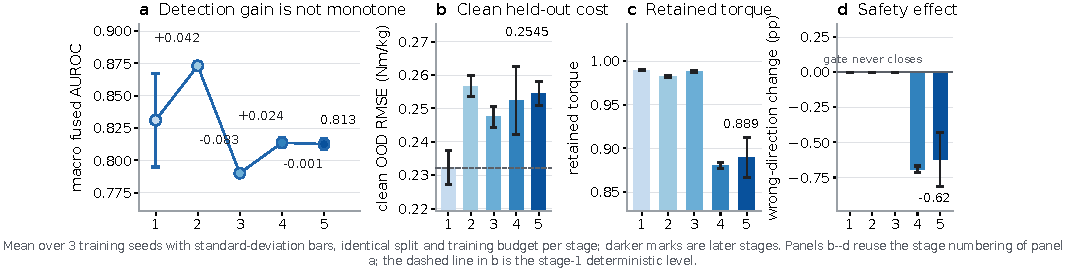
\includegraphics[width=\linewidth]{figures/fig_ablation_summary.pdf}
\caption{固定数据划分和训练预算下的顺序组件归因。阶段按 1--5 编号，依次加入故障增强、概率回归、重建和预测，（b）--（d）沿用相同编号。（a）各阶段的宏平均故障 AUROC，并标注相邻阶段的带符号差值。（b）干净 OOD RMSE，虚线为确定性阶段的参考水平。（c）各阶段在其自身验证选定门控下的保留同向力矩，（d）为对应的反向力矩变化（百分点），两者均在固定故障集合上取宏平均。前三个阶段选出的死区从未被其风险超过，门控因此始终不关闭，面板（d）在这三个阶段恒等于 $0$：此时检测质量对执行没有影响。数值为三个训练种子的均值，误差棒为跨种子标准差。}
\label{fig:ablation-zh}
\end{figure}

每个阶段都用三个种子训练，相邻阶段的差值按种子配对后再统计标准差，因此阶段效应可以与训练随机性直接比较，而不是只看单次运行。故障增强使宏平均故障 AUROC 变化 $+0.042 \pm 0.036$，干净 OOD RMSE 变化 $+0.025 \pm 0.008$ Nm/kg。该 AUROC 变化与确定性阶段本身的种子离散度（$0.831 \pm 0.036$）同量级，因此第一步仍只作为诊断证据，不构成确定的排序。依次加入概率预测、重建和预测分支后，AUROC 分别变化 $-0.083 \pm 0.003$、$+0.024 \pm 0.004$ 和 $-0.001 \pm 0.008$；前两项比种子噪声大一个数量级，最后一项则落在噪声之内。只看检测质量会把阶段 2 排在最前，但面板（d）显示前三个阶段完全没有安全收益：每个阶段从自身验证风险里选出的死区都不会被其测试风险超过，于是 $g_t\equiv1$，反向力矩变化在所有评测场景中恰好为 $0$，保留力矩相应地接近 $0.99$。只有当重建残差进入风险后门控才会关闭，此时反向力矩变化为 $-0.69\pm0.02$ 个百分点，保留力矩为 $0.881 \pm 0.003$；加入预测后该效应保持在 $-0.62\pm0.19$ 个百分点，保留力矩为 $0.889 \pm 0.023$。因此仅按 AUROC 读消融会推举一个对控制无效的配置，这也是归因必须与执行结果一起报告的原因。

\begin{table}[t]
\centering
\small
\setlength{\tabcolsep}{4pt}
\begin{tabular}{lcccc}
\toprule
模型 & RMSE & AUC & 反向差值 & 保留率\\
\midrule
确定性模型 & $0.2322{\pm}0.0051$ & $0.831{\pm}0.036$ & $0.0000$ & $0.990{\pm}0.001$\\
+ 故障增强 & $0.2567{\pm}0.0031$ & $0.873{\pm}0.003$ & $0.0000$ & $0.982{\pm}0.001$\\
+ 概率预测头 & $0.2475{\pm}0.0031$ & $0.790{\pm}0.001$ & $0.0000$ & $0.988{\pm}0.001$\\
+ 重建 & $0.2524{\pm}0.0102$ & $0.814{\pm}0.004$ & $-0.0069{\pm}0.0002$ & $0.881{\pm}0.003$\\
+ 预测（本文模型） & $0.2545{\pm}0.0036$ & $0.813{\pm}0.004$ & $-0.0062{\pm}0.0019$ & $0.889{\pm}0.023$\\
\bottomrule
\end{tabular}
\caption{按顺序进行的组件归因。故障 AUC 和控制指标在固定故障集合上取宏平均，所有行使用相同的数据划分和训练预算。每行为三个训练种子的均值 $\pm$ 标准差（$n=3$）。}
\label{tab:ablation-zh}
\end{table}

故障强度扫描比单一工作点提供了更严格的测试。图~\ref{fig:stress-zh} 汇总两个强度极值以及留一参与者迁移结果。在最大丢包率下，融合 AUROC 在 ID 和 OOD 任务上分别为 $0.961$ 和 $0.914$；相应保留辅助分别为 $0.939$ 和 $0.938$，反向力矩变化分别为 $-0.0007$ 和 $-0.0080$。在最大固定延迟下，融合 AUROC 分别为 $0.899$ 和 $0.788$；门控分别保留 $0.751$ 和 $0.933$ 的同向辅助，并使反向力矩变化 $-0.0132$ 和 $-0.0230$。动作输入消融进一步检验期望、测量、执行或交互力矩能否改善检测，或产生设备专用捷径。在 $25$ 通道仅人体输入的基础上加入这些通道后，ID 宏平均故障 AUROC 仅从 $0.843$ 变为 $0.842$ 至 $0.847$，留出任务从 $0.774$ 变为 $0.771$ 至 $0.784$，而干净 OOD RMSE 从 $0.251$ 升至 $0.259$ 至 $0.278$ Nm/kg。动作反馈既未带来可靠的检测增益，也未出现设备专用捷径应有的「仅 ID 变好」模式，因此保留仅人体输入。若把基于 dropout 的认知不确定性通道替换为同样三个种子构成的三成员深度集成，该通道在 ID 已见故障上的 AUROC 从 $0.497$ 提升到 $0.553$，但融合检测器基本不变（ID 上为 $0.842$ 对 $0.843$，OOD 上均为 $0.771$），因为冻结的融合策略从未选中该通道；干净 RMSE 在三位小数上完全相同。因此集成把推理成本提高到三倍，却没有改变所报告的工作点。15 折留一参与者实验检验该安全效应在人与人之间（而非种子之间）是否稳定。逐参与者的反向力矩降低量平均为 $0.44$ 个百分点，$10{,}000$ 次重采样得到的 $95\%$ bootstrap 置信区间为 $[0.23, 0.67]$ 个百分点，区间不跨过 0，且 $15$ 折全部改善；被试间标准差为 $0.47$ 个百分点，范围为 $0.04$ 至 $1.31$ 个百分点。各折干净条件下的平均保留比例为 $0.961$，最低不低于 $0.880$，说明该降低并非以撤除助力换来。效应在编码器丢帧和延迟故障上最大（ID 上为 $-0.0054$ 和 $-0.0024$，OOD 上为 $-0.0059$ 和 $-0.0094$），在丢包和 IMU 偏置上最小（ID 上为 $-0.0009$ 和 $-0.0008$）。因此参与者迁移在符号上一致，但幅度不大，且在参与者之间相差数倍。

\begin{figure}[t]
\centering
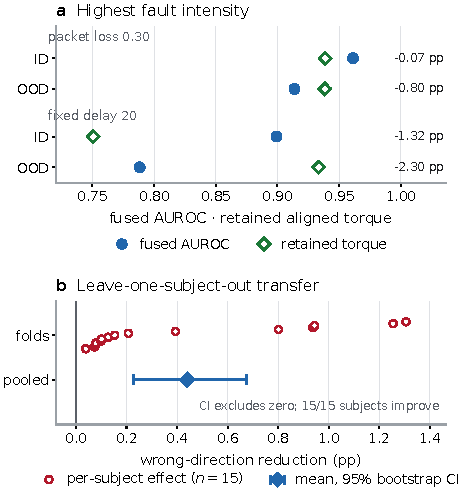
\includegraphics[width=\linewidth]{figures/fig_stress_transfer.pdf}
\caption{强度极值与参与者迁移。（a）在最大丢包率和最长固定延迟下，实心圆为融合 AUROC，空心菱形为保留同向力矩比例，两者共用同一坐标轴；直接标注给出以百分点表示的反向力矩变化。（b）每个空心圆为一折留一参与者结果，菱形给出 $15$ 折的均值及其 $95\%$ bootstrap 置信区间。区间不跨过 0 且每折都改善，说明反向力矩的降低在参与者之间符号一致；但最弱与最强折之间的幅度相差约三十倍。}
\label{fig:stress-zh}
\end{figure}

\section{讨论}

可靠性估计只有在改变指令时才具有实际作用，而不能只作为置信度分数。在主要实验中，验证集标定的门控使非干净条件下的反向辅助绝对值平均减少约 $0.007$，同时保留 $96.1\%$ 的干净同向力矩。这只是一个工作点上的有限改善，并不构成安全保证。不过，该结果并非通过简单关闭辅助获得。AUROC 不衡量控制后果，因此需要同时报告反向力矩和保留辅助才能呈现这种权衡，消融也说明两者可以彼此独立地变化。

不同故障机理破坏的信号性质不同，性能差异也随之较大：重建对鞋垫缺失最有效，停滞性主要检测丢包，一致性主要检测部分通道缺失和延迟。融合覆盖更多情况，但 IMU 偏置仍接近随机水平，说明缓慢偏置可能无法通过现有传感器与有效动作区分。一些辅助头还以明显超过种子噪声的幅度降低了聚合性能，干净 RMSE 也差于划分匹配的确定性 TCN。预测不确定性和辅助训练都不能解决所有传感器故障，仍需更敏感的偏置检查和更合适的损失平衡。

本文方法补充而非替代两条基线研究方向。任务无关估计扩大动作覆盖范围 \citep{molinaro2024task}，领域适应降低训练数据需求 \citep{scherpereel2025domain}，本文门控则处理部署后的损坏观测。领域适应后的估计器可以使用同一监控器，但需要在目标传感器域重新标定。执行器能力或风险容忍度不同的应用也应在验证集权衡曲线上重新选择工作点，而不是直接复用本文阈值。

\section{局限性}

所报告的降幅不能全部归因于故障检测。在不存在故障的干净留出任务试验上，门控仍使反向力矩降低 $0.74$ 个百分点，与故障留出试验上的 $1.09$ 和 $1.03$ 个百分点同量级。风险通道对预测误差本身有反应，因此聚合效应中有一部分抑制的是普通的任务偏移误差而非传感器故障；要把两者分开，需要一个当前协议无法隔离的无故障 OOD 对照条件。实验故障均为合成故障，无法覆盖完整的硬件故障分布。我们没有在真实外骨骼上在线运行可靠性门控，也没有进行闭环人体实验。执行器回放假设记录的运动学保持不变，因此只能支持相对比较，不能证明交互安全性、人体适应或代谢收益。力矩标签和传感数据来自单一外骨骼平台，当前实现也没有与 \citet{scherpereel2025domain} 的领域适应模型联合训练。门控可以减少已检测故障的影响，但无法保证未检测或对抗性故障下的安全性，独立的底层力矩和硬件限制仍然必要。

\section{伦理声明}

可靠性感知辅助可能降低静默传感器故障带来的风险，但过度自信的结论可能促使系统在人体环境中过早部署。本文区分离线回放与人体证据，报告负面和较弱的检测结果，并且不把学习得到的门控描述为形式化安全保证。公开参与者数据必须按照来源数据集的条款和知情同意要求处理。

\section{结论}

本文提出一个可靠性层，将学习输出与因果完整性信号结合，并使用验证集标定的风险衰减基于力矩的辅助。实验将参与者、任务和传感器故障偏移分开，同时报告有害力矩的下降和为此损失的辅助。未来工作将改进缓慢偏置检测，并在真实外骨骼人体实验中实时验证完整监控器和回退策略。在该方法用于受控传感器条件之外的任务无关辅助之前，必须完成实时验证。

\bibliographystyle{aaai2027}
\bibliography{references}

\end{document}
